\documentclass[onecolumn]{article}
\usepackage{url}
\usepackage{algorithm}
\usepackage{algorithmic}
\usepackage[a4paper]{geometry}
\usepackage{datetime}
\usepackage[margin=2em, font=small,labelfont=it]{caption}
\usepackage{graphicx}
\usepackage{mathpazo} % use palatino
\usepackage[scaled]{helvet} % helvetica
\usepackage{microtype}
\usepackage{amsmath}
\usepackage{subfigure}
\usepackage[procnames]{listings}
\usepackage{color}


% Letterspacing macros
\newcommand{\spacecaps}[1]{\textls[200]{\MakeUppercase{#1}}}
\newcommand{\spacesc}[1]{\textls[50]{\textsc{\MakeLowercase{#1}}}}

\title{\spacecaps{Lab report: SW01 }\\ \normalsize \spacesc{TSM\_DeLearn} }

\author{Andrin Bürli\thanks{andrin.buerli@hslu.ch}, Nursinem Dere\thanks{nursinem.dere@stud.hslu.ch}, Fabian Gröger\thanks{fabian.groeger@hslu.ch}\\Hochschule Luzern}
\date{\today}

\begin{document}
\maketitle

\definecolor{keywords}{RGB}{255,0,90}
\definecolor{comments}{RGB}{0,0,113}
\definecolor{red}{RGB}{160,0,0}
\definecolor{green}{RGB}{0,150,0}


\lstset{language=Python, 
	basicstyle=\ttfamily\small, 
	keywordstyle=\color{keywords},
	commentstyle=\color{comments},
	stringstyle=\color{red},
	showstringspaces=false,
	identifierstyle=\color{green},
	procnamekeys={def,class}}


\section{Introduction}

In the first week of Deep Learning (TSM\_DeLearn) course, McCulloch-Pitts Neuron, Rosenblatt's Perceptron and Perceptron Learning, ANN(Single Layer LTU, Multi Layer Perceptron) concepts and etc. are introduced with examples. The solutions of exercises are included in the next section of this report.

\section{Exercise 3: Perceptron Learning Algorithm}

A perceptron is a classification model that consists of a set of weights, or scores, one for every feature, and a threshold. The perceptron multiplies each weight by its corresponding score, and adds them, obtaining a score. If this score is greater than or equal to the threshold, then the perceptron returns the value 1. If it is smaller, then it returns the value 0.

\begin{algorithm}[H] 
	\caption{Perceptron Learning Algorithm}
	\begin{enumerate}
		\item
		Initialize the weights as zero
		\item
		Iterate by updating weights according to:
		\begin{enumerate}
			\item
			Pick a sample $(x^{(i)}, y^{(i)})$
			\item
			Compute predicted values: $y^{(i)} = H(w.x^{(i)}+b)$
			\item
			Parameter update rule: only update if $y^{(i)} \neq  \hat{y}^{(i)}$
			\begin{enumerate}
				\item
				$w \leftarrow w - \alpha (y^{(i)} - \hat{y}^{(i)})x^{(i)}$
				\item
				$b \leftarrow b - \alpha (y^{(i)} - \hat{y}^{(i)})$
			\end{enumerate}
		\end{enumerate}
		
	\end{enumerate}
\end{algorithm}

\subsection{Step 1: Low-Dimensional Dataset}

In the first step, Rosenblatt Perceptron is implemented to a low dimensional dataset with the perceptron learning rule to separate the dataset linearly.\newline
First we define a dataset with 200 samples where 100 of them labeled as 1.  \newline
\begin{lstlisting}
x,y = prepare_data(200,100,0,0.5,width=0.3,eps=0.5, seed=1)
plot(x, y, params_before=(0,0.5))  
\end{lstlisting}
To find the decision boundary to separate the dataset, implement a function that translates the weights vector (w$_{1}$, w$_{2}$) and the bias $b$  into parameters of a straight line (x$_{2}$ = a + s . x$_{1}$).
\begin{lstlisting}
def lineparams(weight, bias): 
	a = -bias / weight[0,1]
	s = -weight[0,0] / weight[0,1]  
return a,s
\end{lstlisting}
To implement the perceptron learning algorithm, predict, update, select\_datapoint and train functions are used.
The function below returns the predicted value for a perceptron.
\begin{lstlisting}
def predict(x,w,b): 
	y = np.heaviside((np.dot(w,x) + b),1)
return y
\end{lstlisting}
The function below performs an update step in accordance with the perceptron learning algorithm.
\begin{lstlisting}
def update(x,y,w,b,alpha=1.0): 
	ypred = predict(x,w,b)
	w1 = w - alpha*(ypred-y)*x
	b1 = b - alpha*(ypred-y)  
return w1, b1
\end{lstlisting}
The function below identifies the misclassified data points and selects one of them. In case all datapoints are correctly classified None is returned.
\begin{lstlisting}
def select_datapoint(x, y, w, b): 
	ypred = predict(x,w,b)
	wrong_mask = (ypred != y)[0]
	misclassified = np.where(wrong_mask)[0]
	if len(misclassified)>0:
		x1 = x[:,misclassified[0]]
		y1 = y[0,misclassified[0]]
	return x1, y1, misclassified
return None, None, []
\end{lstlisting}
The function below trains the perceptron (single LTU) for the given data x and ground truth labels y by using the perceptron learning algorithm with learning rate alpha (default is 1.0).
\begin{lstlisting}
def train(weight_init, bias_init, x, y, alpha=1.0,
debug=False, params_best=None, max_iter=1000):
	weight = weight_init
	bias = bias_init
	iterations = 0
	misclassified_counts = [] 
	while iterations<=max_iter:
		x1, y1, misclassified = select_datapoint(x,y,weight,bias)
		misclassified_counts.append(len(misclassified))
		if len(misclassified)==0:
			return weight, bias, misclassified_counts
		params_before = lineparams(weight, bias)
		weight,bias = update(x1,y1,weight,bias,alpha)
		iterations = iterations + 1
return weight, bias, misclassified_counts
\end{lstlisting}
To test the implementation, a dataset with 100 data points(50 of them labeled as 1), 0 as the initial value a, 0 as the initial value s is defined and training run with the default learning rate($\alpha$ = 1), where weights are [0 1] and the bias is 0.\newline
\begin{figure}[h]
	\centering
	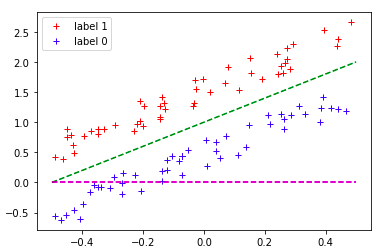
\includegraphics[width=.4\linewidth]{fig/initial.png}
	\caption{\label{fig:initial}
		Initial decision boundary}
\end{figure}\newline 
And after 29 iteration, best parameters as the solution found by perceptron learning rule are the weights [-4.99046876  2.92867787] as the bias is -3.

\begin{figure}[h]
	\centering
	\subfigure[Decision boundary after the final updates]{\centering
		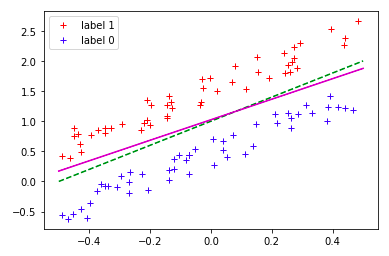
\includegraphics[width=.4\linewidth]{fig/final.png}
		\label{fig:final}}
	\subfigure[Number of iterations]{\centering
		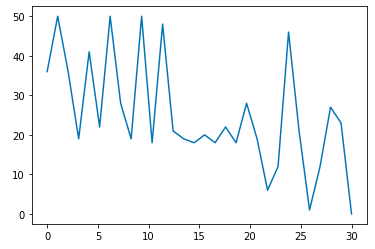
\includegraphics[width=.4\linewidth]{fig/iteration.png}
		\label{fig:iteration}}
	\caption{\label{fig:solution} 
		Results of the performed Perceptron Learning Algorithm }
\end{figure}

\subsection{Step 2: Lightweight MNIST Dataset}

In the second part, same algorithm and functions are applied on MNIST dataset which consists of small (8x8) images, i.e. 64 dimensional arrays. Here, the linear separability can no longer be easily visualized.\newline
For the predict\_digit function predict, for the update\_weights function update, for the select\_digit function select\_datapoint and for the train\_weights function train used as they are introduced in the previous section.\newline
To initialize the parameters, 1x64 zero matrix as weights and bias as 0 are assigned.\newline
After 26 iterations, the final update on the weights and the bias values can be seen below.

\begin{figure}[h]
	\centering
	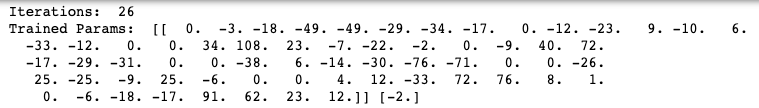
\includegraphics[width=.8\linewidth]{fig/updates_mnist.png}
	\caption{\label{fig:updates_mnist}
		Final values of the weights and the bias.}
\end{figure}

\begin{figure}[h]
	\centering
	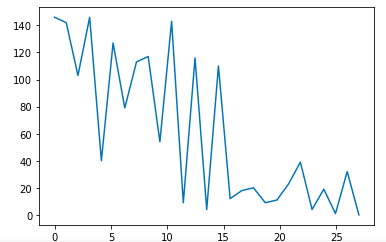
\includegraphics[width=.4\linewidth]{fig/iterations_mnist.png}
	\caption{\label{fig:iterations_mnist}
		Number of iterations}
\end{figure}


\section{Exercise 4: Data Visualization}
The iris species classification task is a classical one. The goal is to distinguish three kinds of iris : setosa, versicolor and virginica. In the data set, a botanist has extracted 4 features : sepal length, sepal width, petal length and petal width.

\begin{lstlisting}
import matplotlib.pyplot as plt 
import seaborn as sns 
import statistics 
iris_data = pd.read_csv('iris.txt', delimiter = "\t")
iris_data1 = iris_data[['Sepal.Length','Sepal.Width',
'Petal.Length','Petal.Width', 'Species']]
ax = sns.pairplot(iris_data1,hue="Species",diag_kind="hist", palette = 'husl')
plt.show()
\end{lstlisting}
It is easier to distinguish setosas (pink circles) from the other two classes by checking their petal length. By assigning a threshold for this variable, it is easy to say that smaller values more likely to belong to the class of setosas. \newline
The other two classes versicolor and virginica can be separated by their petal width as the data points belong to the class virginica mostly have larger petal width than the class versicolor.
\begin{figure}[H]
	\centering
	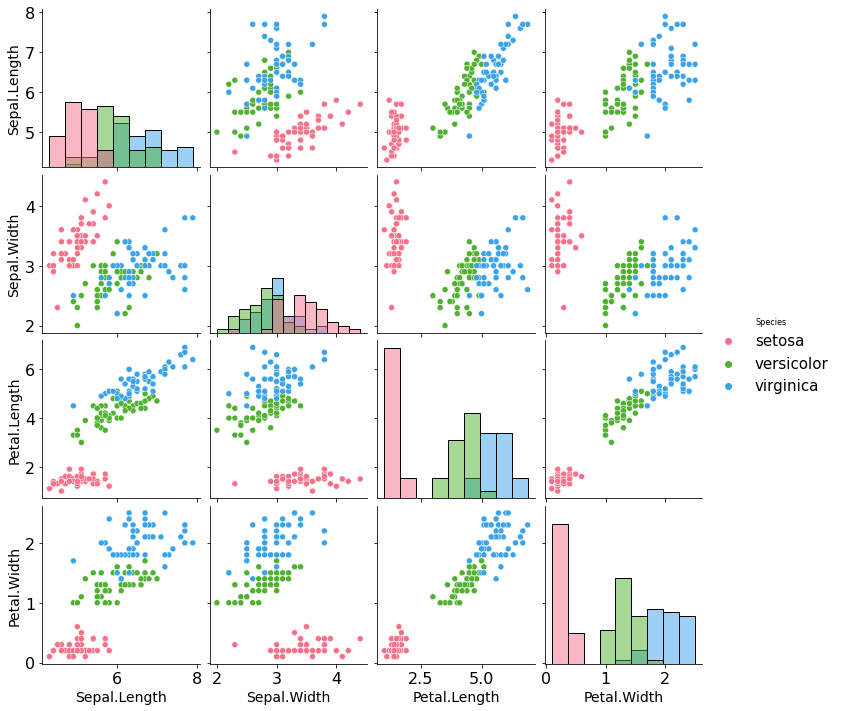
\includegraphics[width=.8\linewidth]{fig/s01_ex4_output.png}
	\caption{\label{fig:s01_ex4_output}
		Final values of the weights and the bias.}
\end{figure}


\section{Exercise 5: Review Questions}

\begin{enumerate}
\item  \textbf{Supervised vs. unsupervised systems}\newline
Of the following examples, which one would you address using a supervised or an unsupervised learning algorithm ? Give some explanations for your answers.
	\begin{enumerate}
		\item \textit{Given email labeled as spam/not spam, learn a spam filter.}\newline Supervised Learning, binary classification where spam and not spam are the two classes of the output.
		\item \textit{Given a set of news articles found on the web, group them into sets of related articles.}\newline Unsupervised learning
		\item \textit{Given a database of customer data, automatically discover market segments and group customers into different market segments.}\newline Unsupervised learning
		\item \textit{Given a dataset of patients diagnosed as either having glaucoma or not, learn to classify new patients as having glaucoma or not.}\newline Supervised learning
	\end{enumerate}	
\item \textbf{Classification vs. regression systems}\newline
\textit{Can we transform a regression problem into a classification problem? What would be the benefits of doing so ?}\newline Regression problem can be transformed to classification problem easily by using binning the predictions. First by replacing the Gaussian distribution for y with a Bernoulli distribution for the case when the response is binary, secondly pass a function that ensures the output in [0,1] which refers to sigmoid function, also known as the logistic or logit function. 
\item \textbf{Perceptron}
	\begin{enumerate}
		\item \textit{For what kind of problems are Perceptrons suited?}\newline The perceptron can only learn simple problems and only useful if the problem is linearly separable.
		\item \textit{For what kind of problems will the Perceptron Learning Algorithm converge?}\newline The perceptron learning algorithm is a linear classifier. If your data is separable by a hyperplane, then the perceptron will always converge. It will never converge if the data is not linearly separable.
		\item \textit{What kind of models can be trained by the Perceptron Learning Algorithm?}\newline The algorithm can be used in separable binary classification problems.
		\item \textit{Give an example for which the Perceptron Learning Algorithm will not converge. Explain why not.}\newline The algorithm does not converge when applied to a non-linearly separable data set.
	\end{enumerate}	
\end{enumerate}

\nocite{*}
\bibliographystyle{plain}
\end{document}

